\onehalfspacing %Para um espa�amento de 1,5
\chapter{Introdu��o}\label{Intro}

Revis�o bibliografica dos principais.

Umas figura de Exemplo:

\begin{figure}[H]
        \begin{center}               
							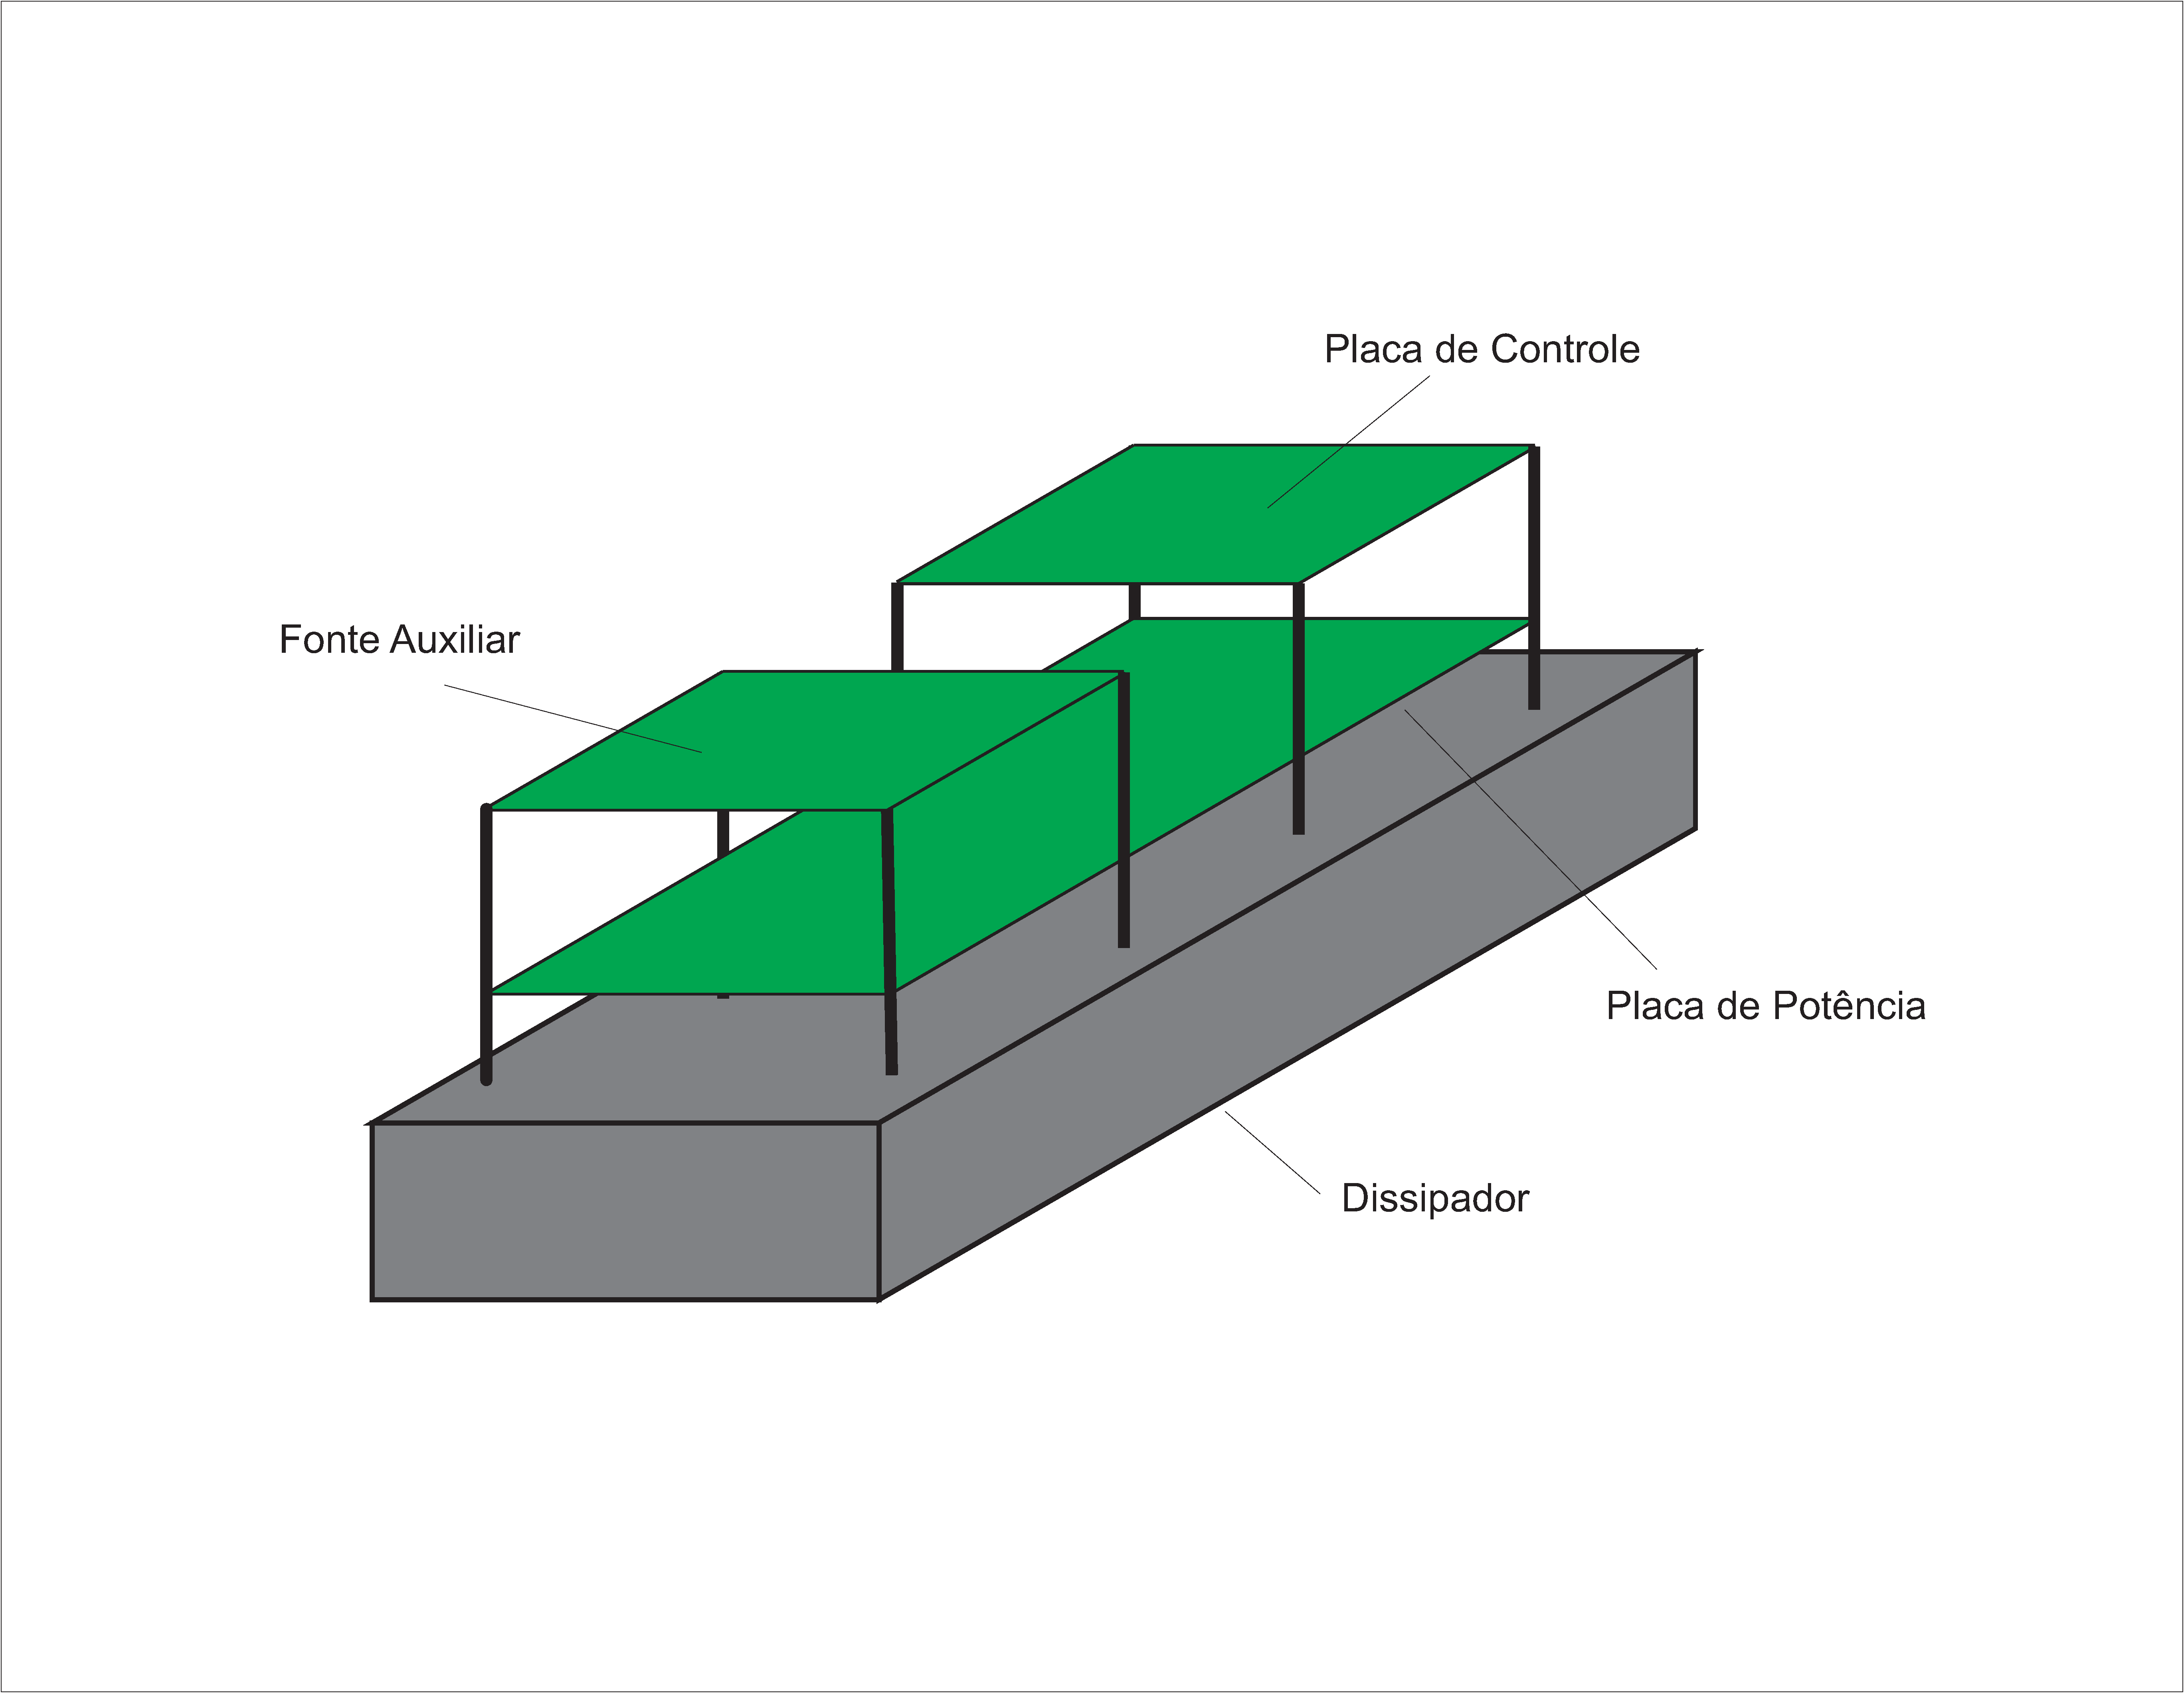
\includegraphics[width=\columnwidth]{Capitulos/01/figs/Designprototipov2.pdf}
        \end{center}
        \caption{Design de um arm�rio.}
        \label{fig:Intro:armario}
\end{figure}

O arm�rio indicado na figura \ref{fig:Intro:armario} tem um design bem interessante, segundo \cite{lem}.

Uma tabelinha bem legal.

\begin{table}[H]
	\renewcommand{\arraystretch}{1.2}
	\caption{Descri��o dos vetores do Retificador de Tens�o Trif�sico.}
	\vspace{-12pt}
	\label{CHmod_tab_estados}
	\centering
	\small
	\begin{center}
		\begin{tabular}{  c | c | >{\centering}p{0.45cm} | >{\centering}p{0.45cm} | >{\centering}p{0.45cm} | >{\centering}p{0.45cm} | >{\centering}p{1cm} | c }
			\hline
			\hline
			\multirow{3}{0.7cm}{\centering{Vetor}} &\multirow{3}{1.8cm}{\centering{Interruptores em condu��o}} & \multicolumn{5}{c|}{Correntes de Entrada} & \multirow{3}{*}{Forma Polar} \\
			\cline{3-7}
			 & & \multicolumn{3}{c|}{$abc$} & \multicolumn{2}{c|}{$\alpha\beta$} & \\
			\cline{3-7}
			& & $i_a$ & $i_b$ & $i_c$ & $i_\alpha$ & $i_\beta$ & \\
			\hline
 			${\vec I_1}$ & $S_1$,$S_6$  & {$I_o$} & {$0$}   & {$-I_o$} &  {$I_o$}   & {$\frac{{\sqrt 3 }}{3}{I_o}$} & $\frac{{2\sqrt 3 }}{3}{I_o}\angle {30^ \circ }$
 			\\
 			${\vec I_2}$ & $S_2$,$S_6$  & {$0$}   & {$I_o$} & {$-I_o$} &  {$0$}   & {$\frac{{2\sqrt 3 }}{3}{I_o}$} & $\frac{{2\sqrt 3 }}{3}{I_o}\angle {90^ \circ }$
 			\\
 			${\vec I_3}$ & $S_2$,$S_4$  & {$-I_o$} & {$I_o$}   & {$0$} &  {$-I_o$}   & {$\frac{{\sqrt 3 }}{3}{I_o}$} & $\frac{{2\sqrt 3 }}{3}{I_o}\angle {150^ \circ }$
 			\\
 			${\vec I_4}$ & $S_3$,$S_4$  & {$-I_o$} & {$0$}   & {$I_o$} &  {$-I_o$}   & {$-\frac{{\sqrt 3 }}{3}{I_o}$} & $\frac{{2\sqrt 3 }}{3}{I_o}\angle {-150^ \circ }$
 			\\
 			${\vec I_5}$ & $S_3$,$S_5$  & {$0$}    & {$-I_o$}   & {$I_o$} &  {$0$}   & {$-\frac{{2\sqrt 3 }}{3}{I_o}$} & $\frac{{2\sqrt 3 }}{3}{I_o}\angle {-90^ \circ }$
 			\\
 			${\vec I_6}$ & $S_1$,$S_5$  & {$I_o$} & {$-I_o$}   & {$0$} &  {$I_o$}   & {$-\frac{{\sqrt 3 }}{3}{I_o}$} & $\frac{{2\sqrt 3 }}{3}{I_o}\angle {-30^ \circ }$
 			\\
 			\hline 
 			\multirow{3}{*}{${\vec I_0}$} & $S_1$,$S_4$  & \multirow{3}{*}{0}   & \multirow{3}{*}{0}   & \multirow{3}{*}{0} &  \multirow{3}{*}{0}   & \multirow{3}{*}{0} & \multirow{3}{*}{$0\angle {0^ \circ }$}
 			\\
 			& $S_2$,$S_5$  & & & & & &
 			\\
 			 & $S_3$,$S_6$  & & & & & &
 			\\ 	 		 			
 			\hline
			\hline
		\end{tabular}
	\end{center}
\end{table}

Outra mais simplezinha.

\begin{table}[H]
	\renewcommand{\arraystretch}{1.2}
	\caption{Intervalo de cada um dos setores.}
	\vspace{-8pt}
	\label{CHmod_tab-setores}
	\centering
	\begin{center}
		\begin{tabular}{ c | c }
			\hline
			\hline
			{Setor} & {�ngulo} \\
			\hline
 			1 & $-{30^ \circ }\,a\,\,{30^ \circ }$
			\\
 			2 & ${30^ \circ }\,a\,\,{90^ \circ }$
			\\
 			3 & ${90^ \circ }\,a\,\,{150^ \circ }$
 			\\
 			4 & ${150^ \circ }\,a\,\,{210^ \circ }$
			\\
 			5 & ${210^ \circ }\,a\,\,{270^ \circ }$
			\\
 			6 & ${270^ \circ }\,a\,\,{-30^ \circ }$
			\\
			\hline
			\hline
		\end{tabular}
	\end{center}
\end{table}

%%%%%%%%%%%%%%%%%%%%%%%%%%%%%%%%%%%%%%%%%%%%%%%%%%%%%%%%%%%%%%%%%%%%%%%%%%%%%%%%%%%%%%%%%%%%%%%%%%
%%%%%%%%%%% END OF FILE
%%%%%%%%%%%%%%%%%%%%%%%%%%%%%%%%%%%%%%%%%%%%%%%%%%%%%%%%%%%%%%%%%%%%%%%%%%%%%%%%%%%%%%%%%%%%%%%%%%
